\documentclass[aspectratio=169]{beamer}

\usepackage[utf8]{inputenc}
\usetheme{Madrid}
\usecolortheme{beaver}

\usepackage{graphicx}
\graphicspath{ {./Resources/} }

\title{Project Development Plan}       % Title
\author{Austin, Joe, Matt, Kathryn}                     % Team members
\institute{SNHU/CETA}                                   % Institute
\logo{
\includegraphics[height=0.8cm]{../../AJMK_Logo}}  % Our Logo
\titlegraphic{
\includegraphics[height=2.6cm]{Stencil.png}} % Title graphic

\begin{document}

\frame{\titlepage} % Draw the title page


\begin{frame}
    \frametitle{System Description}

    \begin{block}{Our Goal}
        The goal is to make a PID Demonstrator that teaches the operator how to use a PID loop.
        The operator will have control to adjust each individual variable and see how each effects a
        vertical standing pendulum.
    \end{block}
\end{frame}

\begin{frame}
    \frametitle{Research}

    There are a few different approaches to the PID demonstrator system.

    \begin{columns}

    \begin{column}{0.48\textwidth}
        \begin{block}{Rotary Inverted Pendulum}
             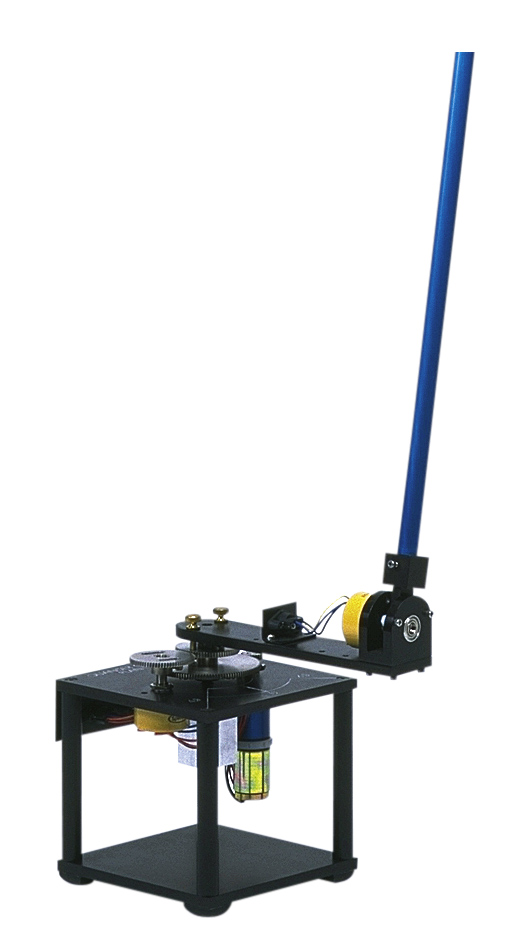
\includegraphics[height=4cm]{RotaryInvertedPendulum}
        \end{block}
        Spins around an axis to produce its motion.
    \end{column}

    \begin{column}{0.48\textwidth}
        \begin{block}{Reaction Wheel Pendulum}
                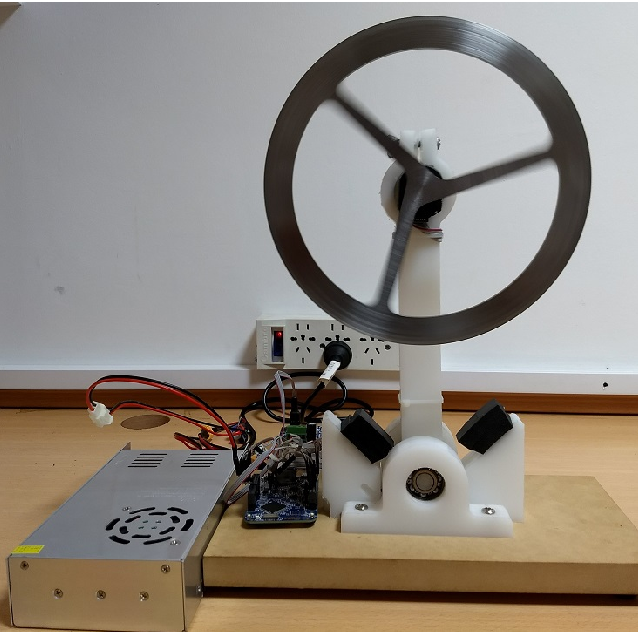
\includegraphics[height=4cm]{ReactionWheel}
        \end{block}
        Uses a reaction wheel to develop a torque against falling over.
    \end{column}
\end{columns}
\end{frame}


\begin{frame}
    \frametitle{System Requirements}

    \begin{columns}
        \begin{column}{0.48\textwidth}
            \begin{block}{Functional Requirements}
                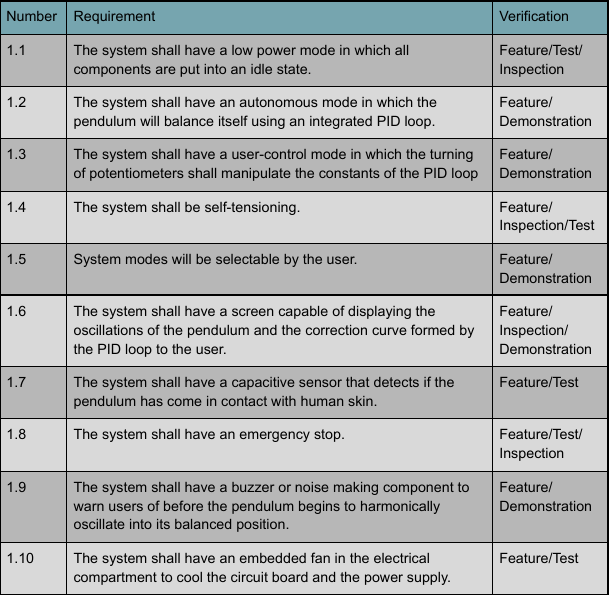
\includegraphics[height=5cm]{FunctionalRequirements}
            \end{block}
        \end{column}

        \begin{column}{0.48\textwidth}
            The functional requirements detail what will make our system, \textbf{our system}. Features
            that are required for us to actually \textbf{solve the problem} we want to solve.
            The most important features include having a \textbf{good user interface mode}, and safety
            systems like an \textbf{emergency stop and gaurds}.
        \end{column}
    \end{columns}
\end{frame}

\begin{frame}
    \frametitle{Risk Assesment}

    \begin{columns}
        \begin{column}{0.48\textwidth}
            Some risks
        \end{column}

        \begin{column}{0.48\textwidth}
            \begin{block}{Risk Assesment}
                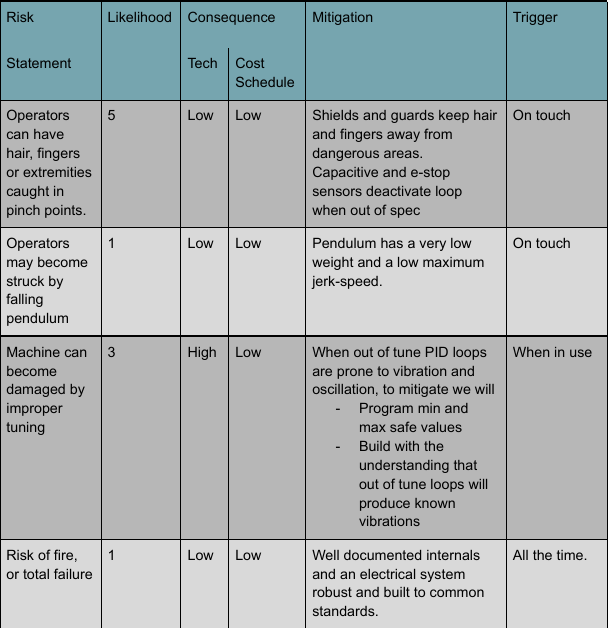
\includegraphics[height=5cm]{RiskAssesment}
            \end{block}
        \end{column}
    \end{columns}
\end{frame}

\begin{frame}
    \frametitle{Design Concepts}
\end{frame}

\begin{frame}
    \frametitle{Task Plan}
\end{frame}

\begin{frame}
    \frametitle{Budget}
\end{frame}

\begin{frame}
    \frametitle{End}

    \begin{block}{}
        \begin{center}
            \Huge Questions and Comments?
        \end{center}
    \end{block}

    \begin{center}
        Find the source code for this document, and the rest of our designs, firmware, hardware
        and notes on GitHub!

        
\includegraphics[height=2cm]{github_qr}
    \end{center}

\end{frame}

\begin{frame}
    \frametitle{References}

    \includegraphics[height=4cm]{references}
\end{frame}


\end{document}
